\documentclass{beamer}
\usetheme{Madrid}
\setbeamertemplate{bibliography item}{\insertbiblabel}

\usepackage[main=english,czech]{babel}
\usepackage[utf8]{inputenc}
\usepackage{url}
\usepackage{caption}

\captionsetup[figure]{font=footnotesize}

%\usepackage{biblatex}
%\addbibresource{references.bib}

\AtBeginSection[]
{
	\begin{frame}<beamer>[noframenumbering]
		\frametitle{Outline}
		\tableofcontents[currentsection]
	\end{frame}
}

\title[Atypic TPC track simul. \& reconstruction]{Simulation and reconstruction of charged particle trajectories in an atypic time projection chamber}
%\subtitle{Subtitle}
\author[M.~Vavřík]{\foreignlanguage{czech}{Martin Vavřík}\vspace{0.5cm}\\martin.vavrik@cvut.cz\\IEAP CTU PRAGUE\\}
\logo{
\includegraphics[width=0.08\textwidth]{../images/logo}}
\date{April 28, 2023}

\begin{document}
	
	\begin{frame}
		\titlepage
	\end{frame}
	
	\begin{frame}
		\frametitle{Outline}
		\tableofcontents
	\end{frame}
	
	\section{Track simulation}
	\begin{frame}
		\frametitle{Track simulation}
		\begin{itemize}
			\item We use Garfield++ for track simulation
			\begin{itemize}
				\item Primary relativistic particle simulated using Heed program~\cite{heed}
				\item Secondary ionization electrons can be simulated using Monte Carlo (gas table calculation necessary)
				\item Alternative approach is microscopic tracking (uses equation of motion)
				\begin{itemize}
					\item A bit slower, more precise especially for small structures.
				\end{itemize}
			\end{itemize}
			\item Currently we have only one track for testing purposes
			\item Soon, more microscopic tracks will be simulated on MetaCentrum to test the reconstruction
		\end{itemize}
	\end{frame}
	
	\begin{frame}
		\frametitle{Simulated track example (microscopic tracking)}		
		\begin{columns}
			\column{0.33\textwidth}
			\begin{figure}
				\centering
				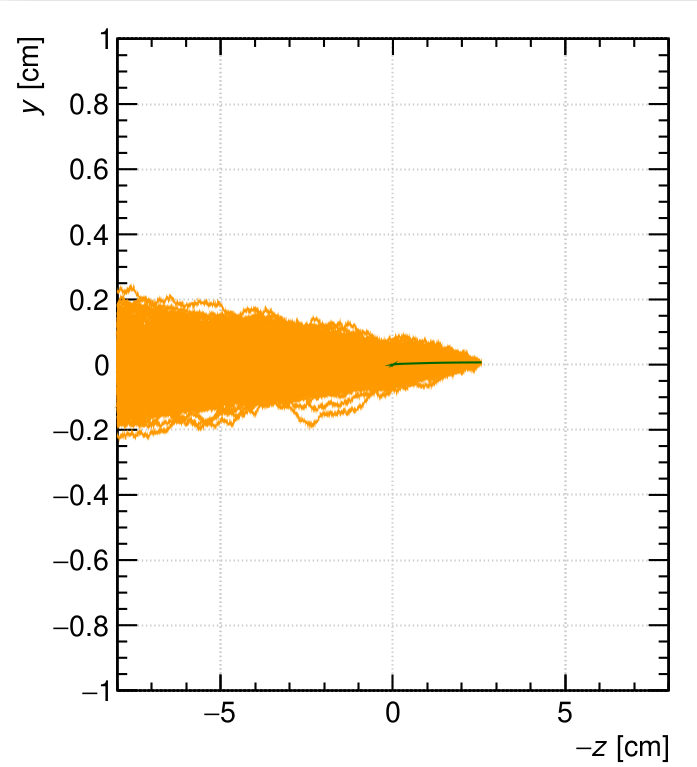
\includegraphics[width = 0.95 \linewidth]{../images/track1.png}
				\caption{Diffusion front view}
			\end{figure}
			\column{0.33\textwidth}
			\begin{figure}
				\centering
				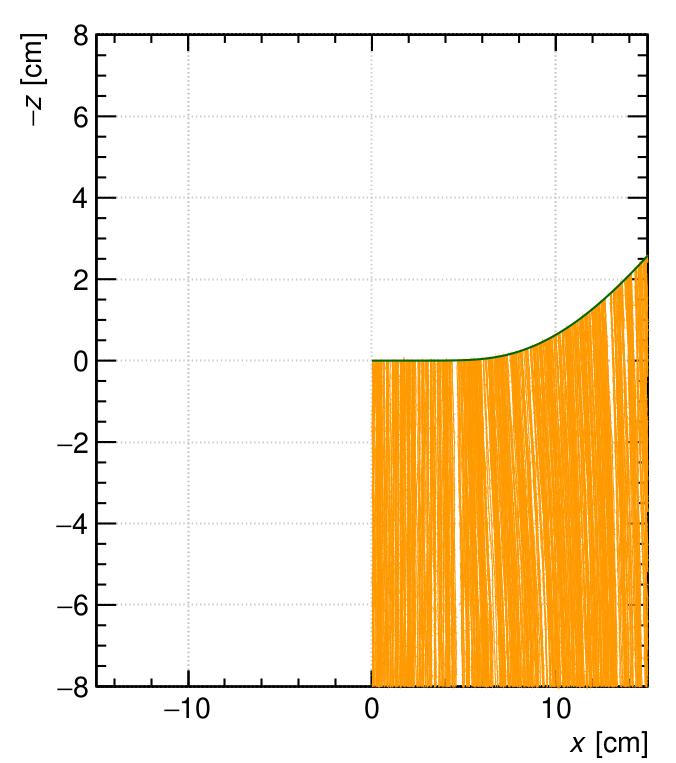
\includegraphics[width = 0.95 \linewidth]{../images/track2.png}
				\caption{Electron drift}
			\end{figure}
			\column{0.33\textwidth}
			\begin{figure}
				\centering
				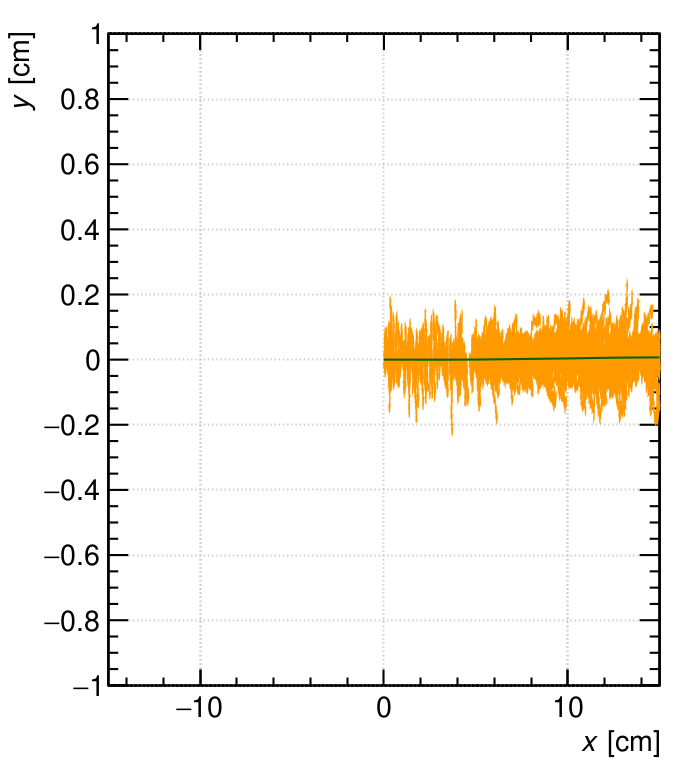
\includegraphics[width = 0.95 \linewidth]{../images/track3.png}
				\caption{Diffusion top view}
			\end{figure}
		\end{columns}
	\end{frame}
	
	\begin{frame}
		\frametitle{Ionization electrons map simulation}
		\begin{itemize}
			\item In the experimental setup TPC detects secondary ionization electrons (after multiplication on triple GEM)
			\item These electrons drift at constant velocity towards the readout plane
			\item We can use simulation of evenly spaced electrons for reconstruction (time consuming -- run on MetaCentrum)
		\end{itemize}
		\begin{figure}
			\centering
			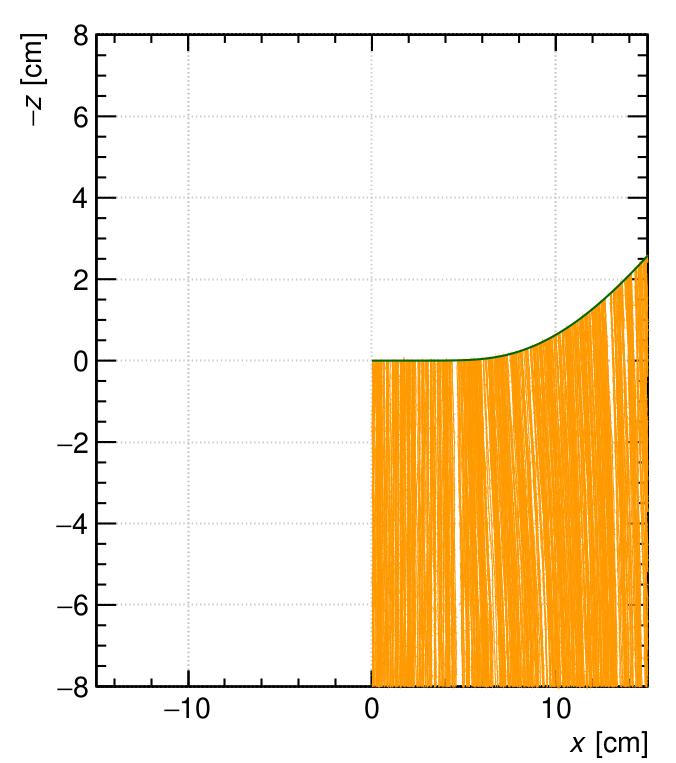
\includegraphics[width = 0.3 \linewidth]{../images/track2.png}
			\caption{Electron drift}
		\end{figure}
	\end{frame}
	
	\begin{frame}
		\frametitle{Ionization electron map simulation}
		\begin{itemize}
			\item As a result we get an approximation of a mapping from initial coordinates of the electrons $(x,y,z)$ to the readout coordinates $(x',y',t)$
			\item By interpolating the resulting readout coordinates (we know the respective initial coordinates) we can get an approximation of the initial coordinates for any point (we get the inverse map)
			\item We can use the inverse map to finally create mapping from our discrete readout values (channel number, time) to voxels of the primary track
		\end{itemize}
		\begin{figure}
			\centering
			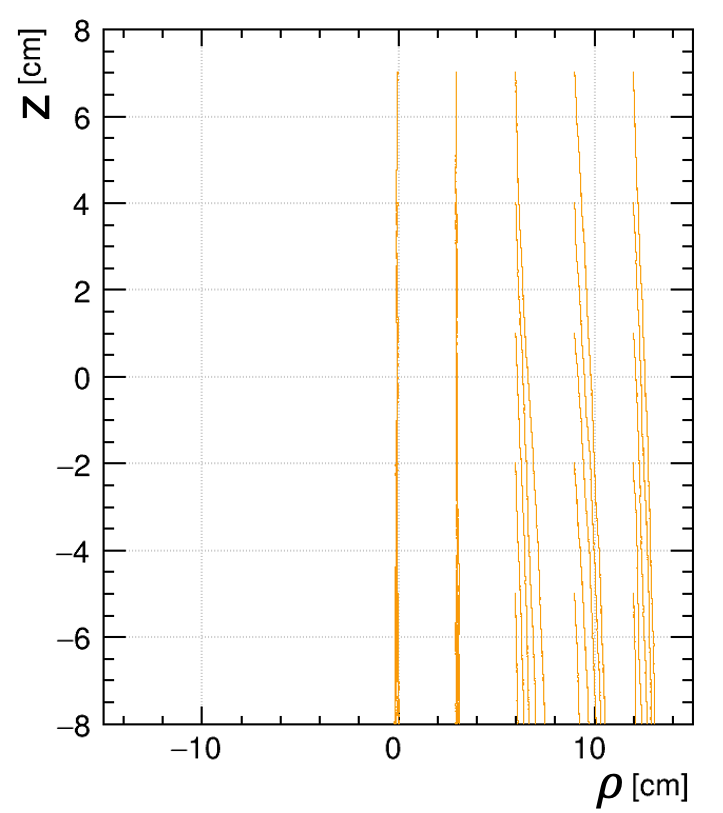
\includegraphics[height=0.4\textheight]{../images/map_lines.png}
			\caption{Partial simulation of the map}
		\end{figure}
	\end{frame}
	\begin{frame}
		\frametitle{Ionization electron map simulation}
		\begin{figure}
			\centering
			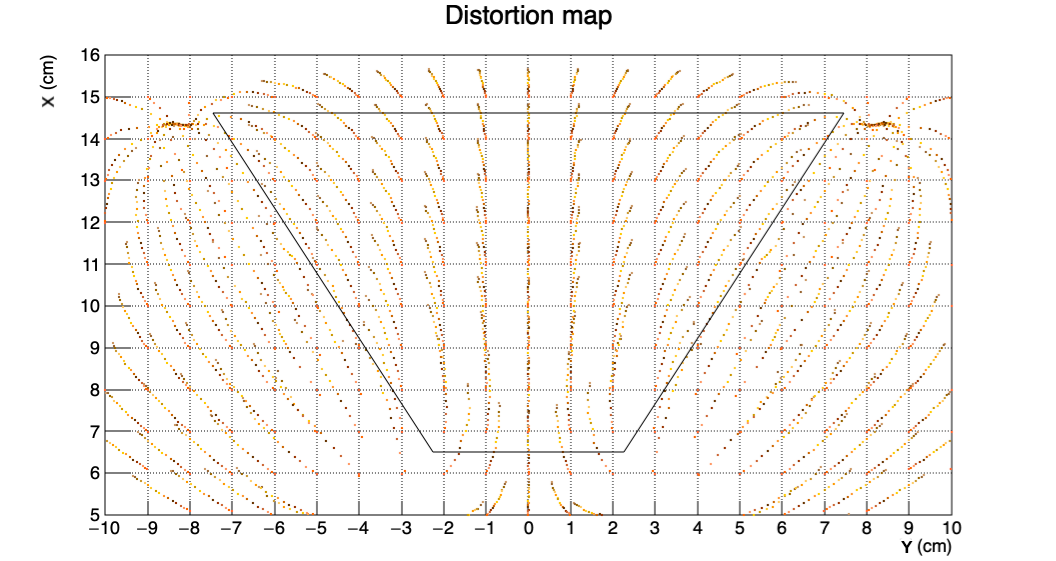
\includegraphics[height=0.6\textheight]{../images/map_dist.png}
			\caption{The average readout coordinates $x$ and $y$ of ionization electrons generated at different $z$ values denoted by color (Credit: Hugo Natal da Luz).}
		\end{figure}
	\end{frame}
	\begin{frame}
		\frametitle{Ionization electron map simulation}
		\begin{figure}
			\centering
			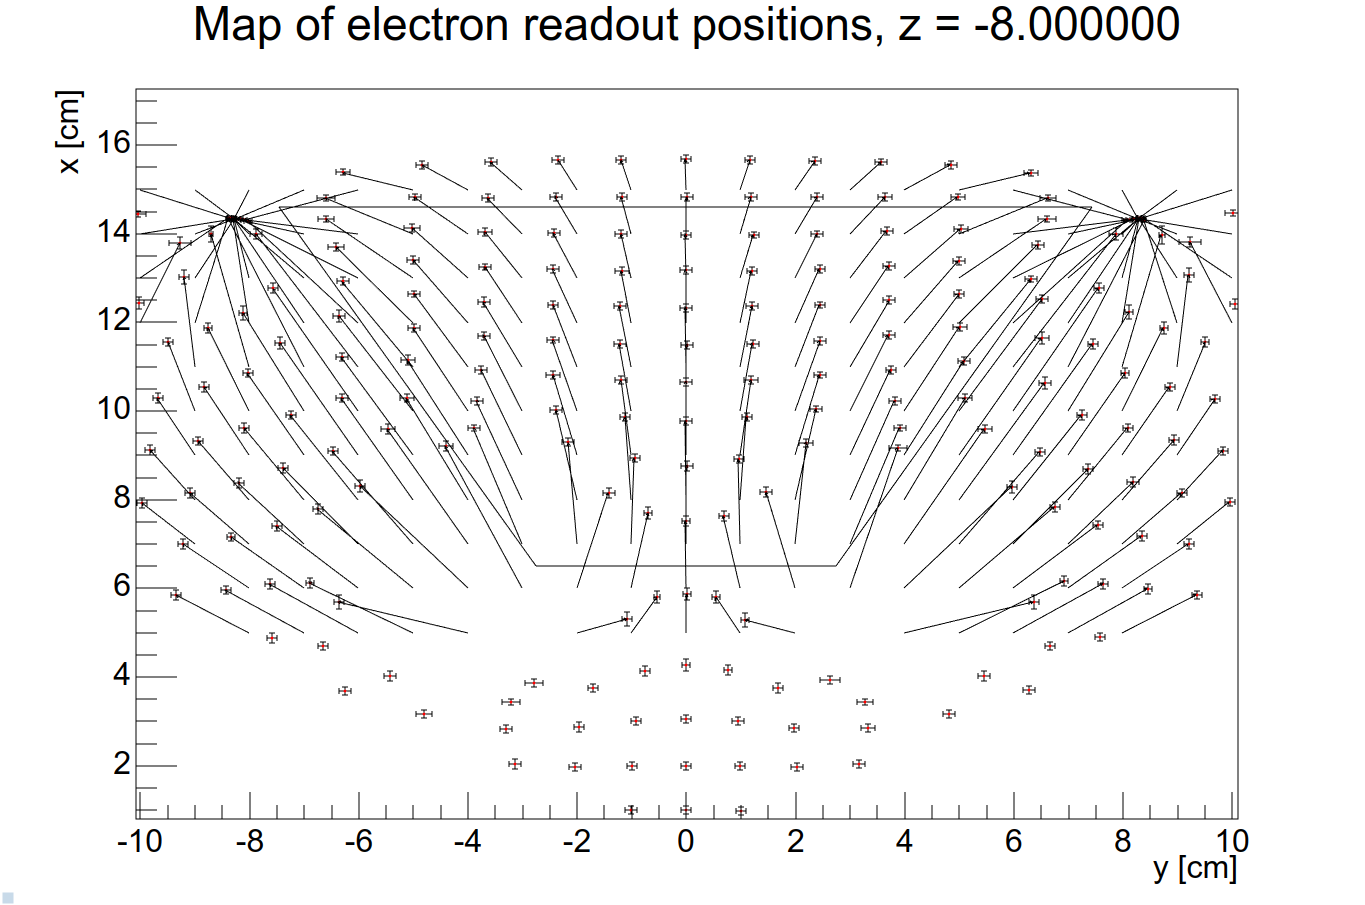
\includegraphics[height=0.65\textheight]{../images/map_dist2.png}
			\caption{The average readout coordinates $x$ and $y$ of ionization electrons generated for maximal initial distance from readout. The tail of each arrow denotes the initial coordinates.}
		\end{figure}
	\end{frame}
	\begin{frame}
		\frametitle{Ionization electron map simulation}
		\begin{figure}
			\centering
			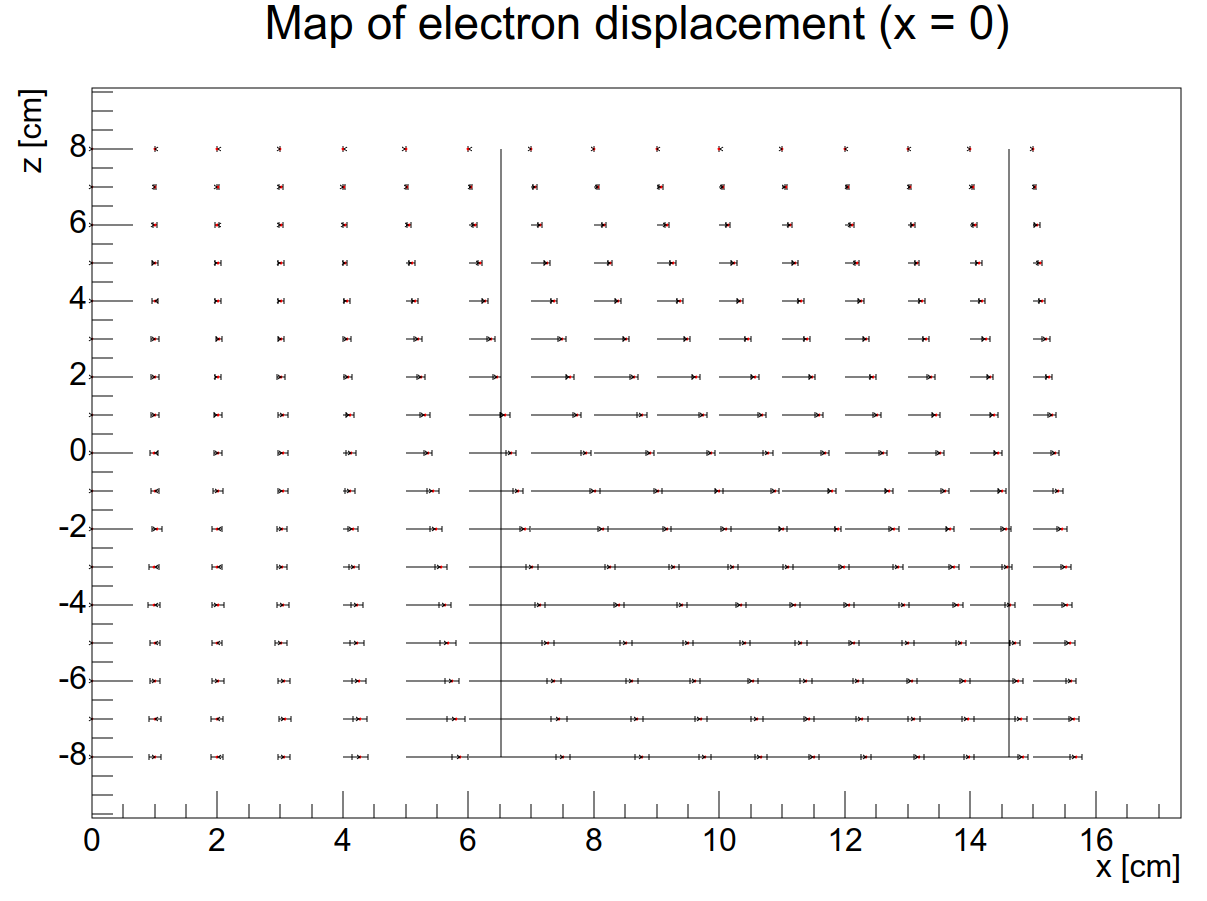
\includegraphics[height=0.65\textheight]{../images/map_xz.png}
			\caption{The average readout x-coordinate of ionization electrons generated for different initial $x$~and $z$~coordinates ($y=0$). The tail of each arrow denotes the initial coordinates.}
		\end{figure}
	\end{frame}
	\begin{frame}
		\frametitle{Ionization electron map simulation}
		\begin{figure}
			\centering
			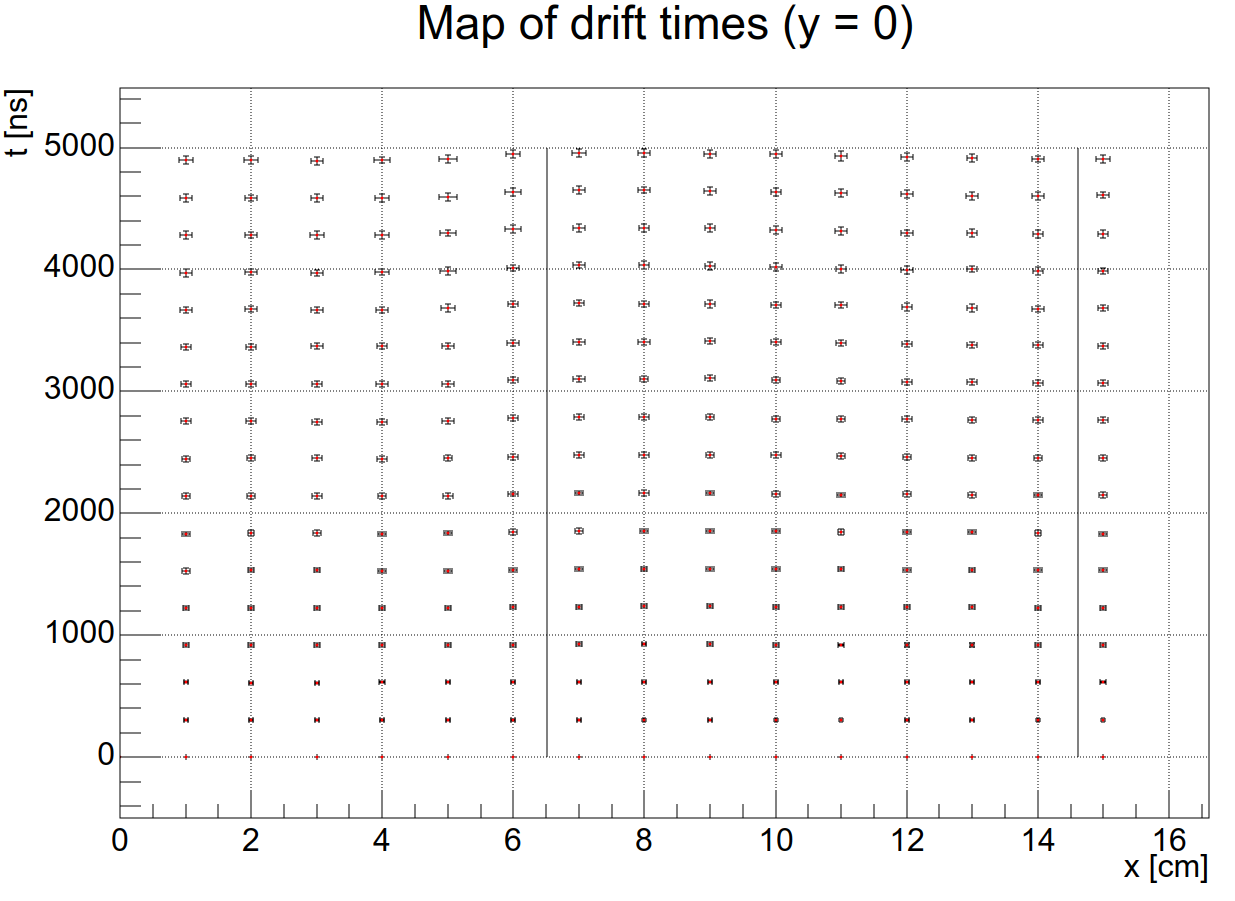
\includegraphics[height=0.65\textheight]{../images/map_xt.png}
			\caption{The average readout coordinates $x$ and $t$ of ionization electrons generated for different initial $x$~and $z$~coordinates ($y=0$).}
		\end{figure}
	\end{frame}
	\begin{frame}
		\frametitle{Ionization electron map simulation}
		\begin{figure}
			\centering
			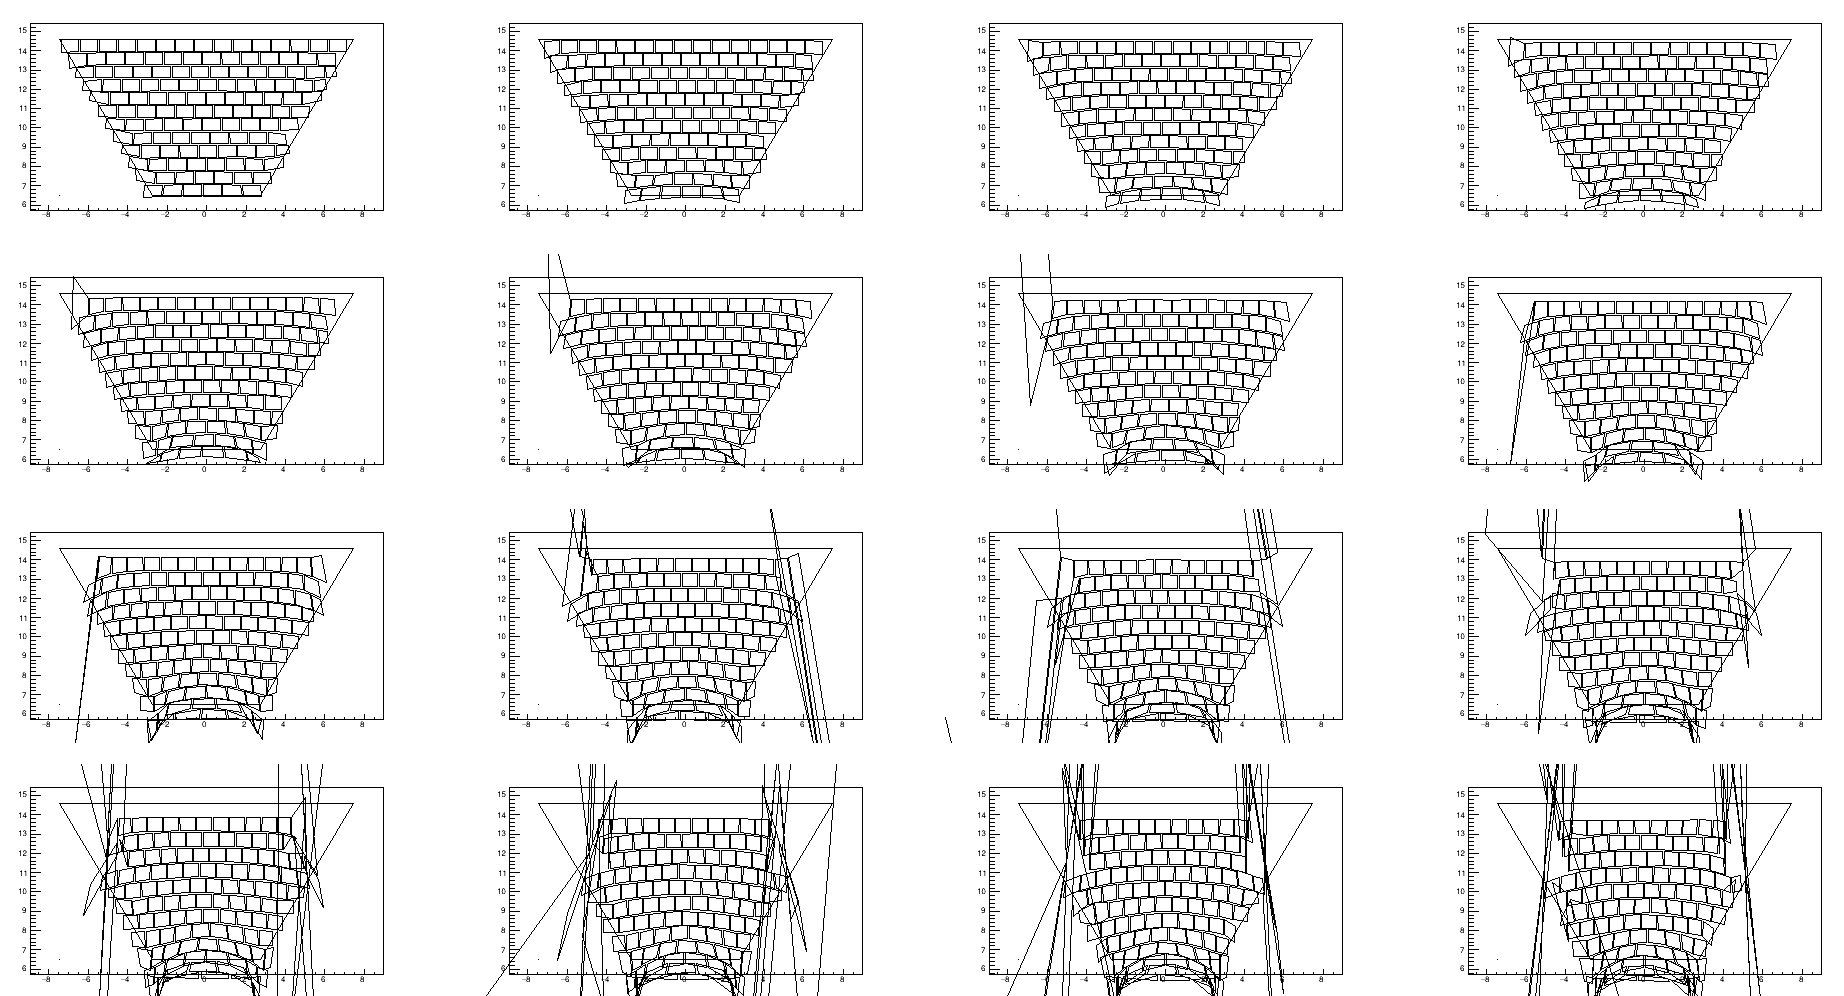
\includegraphics[height=0.68\textheight]{../images/pads_dist.png}
			\caption{Pad voxel boundaries for different times (picture of the first attempt). Errors might be caused by attempted interpolation outside the simulated grid.}
		\end{figure}
	\end{frame}
	
	
	\section{Track reconstruction}
	\begin{frame}
		\frametitle{Track reconstruction}
		\begin{itemize}
			\item Preliminary attempts using the inverse map (not accounting for readout pads - we assume we know the coordinates exactly)
			\item These attempts were used to test the map (see residues on the next slide)
		\end{itemize}
		\begin{figure}
			\centering
			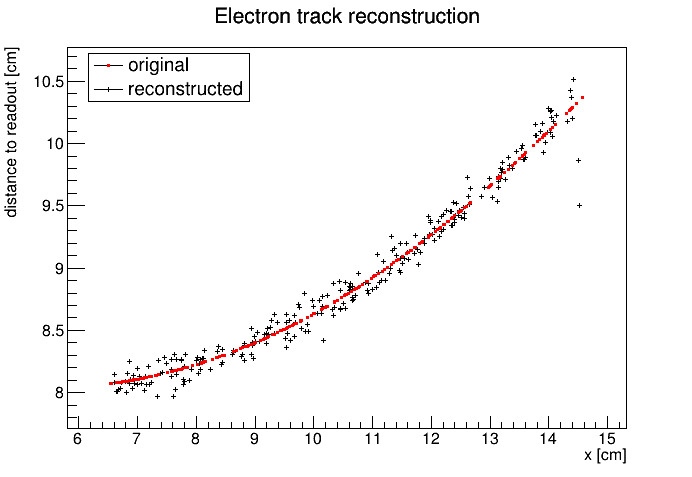
\includegraphics[width=0.6\textwidth]{../images/reco_track.png}
			\caption{Original and reconstructed interaction points on the simulated track}
		\end{figure}
	\end{frame}
	\begin{frame}
		\frametitle{Track reconstruction}
		\begin{figure}
			\centering
			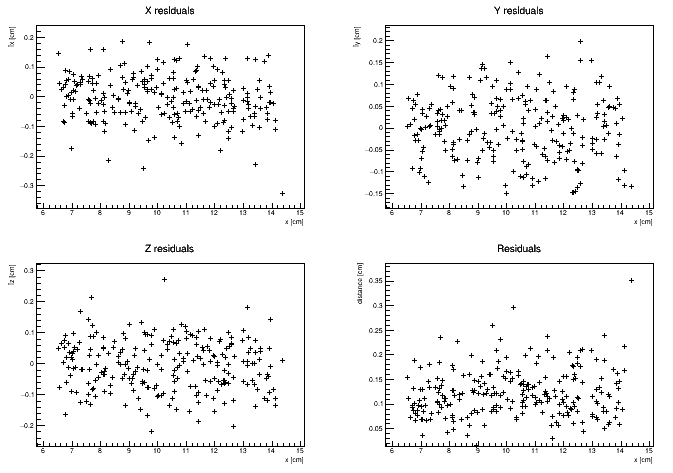
\includegraphics[width=0.6\textwidth]{../images/residues_scatter.png}
			\caption{Residues ($x,y,z$ and combined) of the interaction point reconstruction using the map displayed as~a~scatter plot along the tracks original direction x.}
		\end{figure}
	\end{frame}
	\begin{frame}
		\frametitle{Track reconstruction}
		\begin{figure}
			\centering
			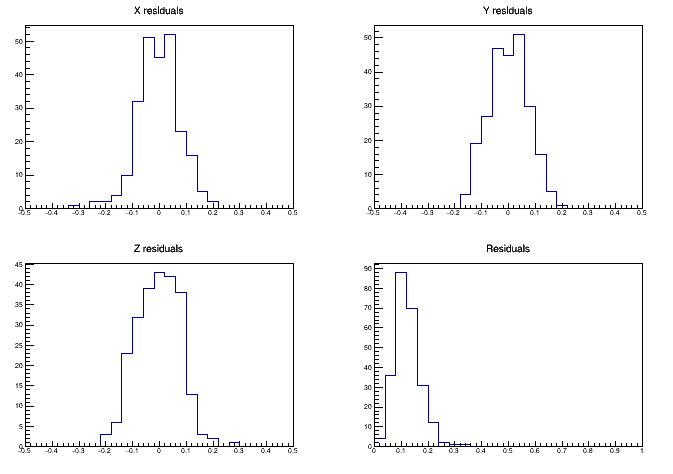
\includegraphics[width=0.6\textwidth]{../images/residues_hist.png}
			\caption{Residues ($x,y,z$ and combined) of the interaction point reconstruction using the map displayed as~a~histogram.}
		\end{figure}
	\end{frame}
	
	\section{Energy reconstruction}
	\begin{frame}
		\frametitle{Energy reconstruction}
		\begin{itemize}
			\item With or without pads
			\item We are counting the number of electrons as charge of the pad
			\item Initial fit with smoothly attached circular arc with straight lines (expected in homogeneous field)
			\begin{itemize}
				\item Fitted parameters:
				\begin{itemize}
					\item radius, direction of bending, starting point of the circle and length of the circle
				\end{itemize}
				\item Orientation and position of the first line is fixed in the fit
				\item The magnetic field in the middle of the chamber (where the track crosses the middle x-coordinate) is used as B value
				\item Reconstruction of energy tested on Runge-Kutta generated tracks with random initial parameters (no pads)
			\end{itemize}
			\item Energy is then refined using the Runge-Kutta 4th order fit (assuming known direction)
		\end{itemize}	
	\end{frame}
	\begin{frame}
		\frametitle{Energy reconstruction}
		\begin{figure}
			\centering
			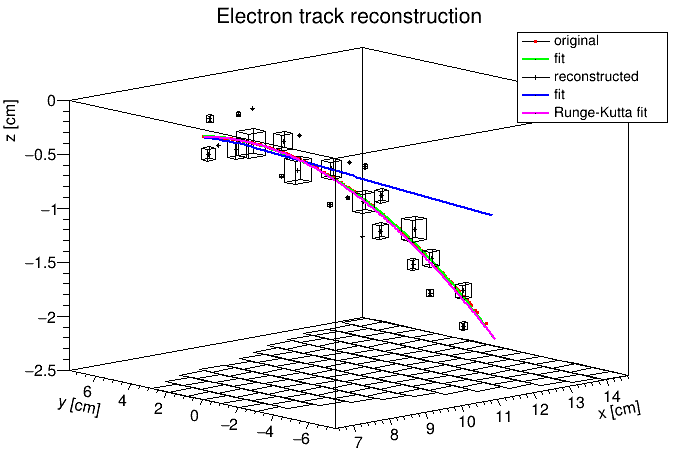
\includegraphics[width=0.55\textwidth]{../images/track_fits.png}
			\caption{Original and reconstructed (with pads) 7.49~MeV track fitted with the lines and circle fit (both original and reconstructed, not yet tuned for pads). Reconstructed track is also fitted by the Runge-Kutta fit. Initial reconstructed energy is 7.55~MeV for the original fit and 8.86~MeV from the reconstructed. Refined energy with Runge-Kutta fit (with pads) is $7.374 \pm 0.037$~MeV.}
		\end{figure}
	\end{frame}
	\begin{frame}
	\frametitle{Energy reconstruction}
		\begin{figure}
			\centering
			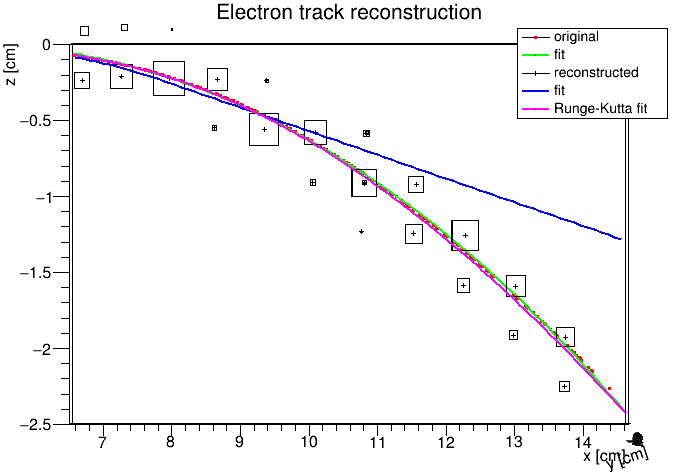
\includegraphics[width=0.49\textwidth]{../images/track_fits_xz.png}
			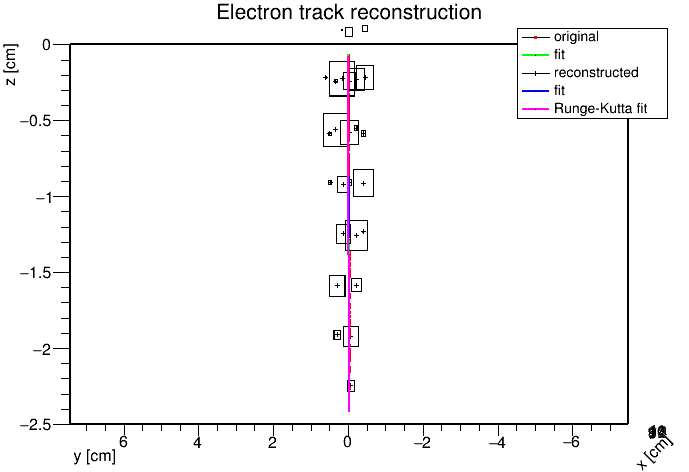
\includegraphics[width=0.49\textwidth]{../images/track_fits_yz.png}
		\end{figure}
	\end{frame}
	\begin{frame}
	\frametitle{Energy reconstruction - circle fit test with Runge-Kutta sample}
		\begin{figure}
			\centering
			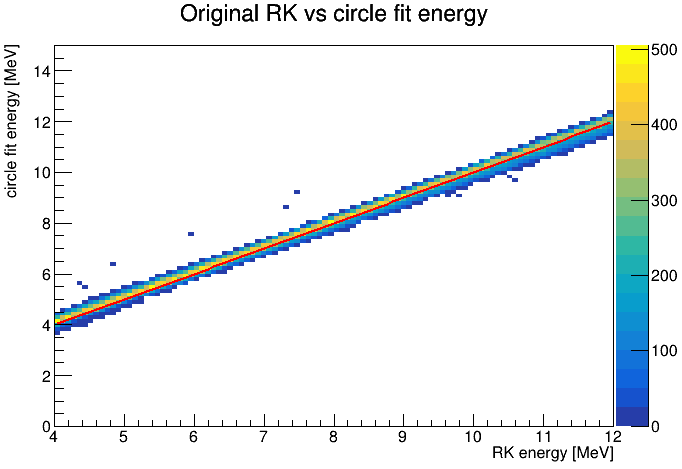
\includegraphics[width=0.55\textwidth]{../images/rk_energy.png}
			\caption{Simulated vs reconstructed energy of the Runge-Kutta generated tracks. Function $y=x$ displayed in red for reference.}
		\end{figure}
	\end{frame}
	\begin{frame}
	\frametitle{Energy reconstruction - circle fit test with Runge-Kutta sample}
		\begin{figure}
			\centering
			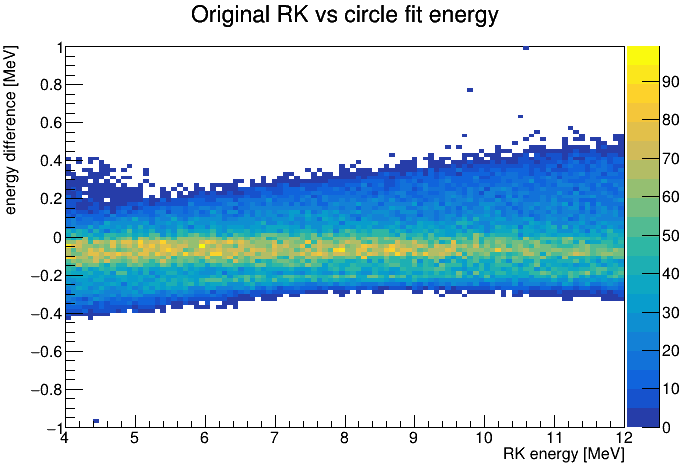
\includegraphics[width=0.55\textwidth]{../images/rk_energy_diff.png}
			\caption{Dependence of the difference in the simulated and reconstructed energy (absolute error) on the simulated energy.}
		\end{figure}
	\end{frame}
	\begin{frame}
	\frametitle{Energy reconstruction - circle fit test with Runge-Kutta sample}
		\begin{figure}
			\centering
			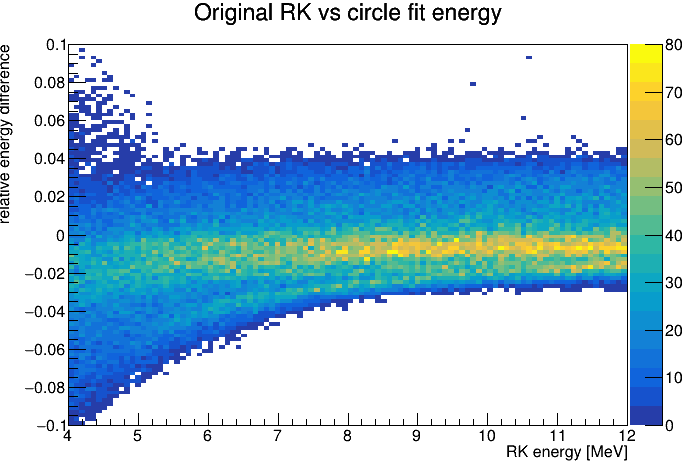
\includegraphics[width=0.55\textwidth]{../images/rk_energy_reldiff.png}
			\caption{Dependence of the relative difference in the simulated and reconstructed energy (relative error) on the simulated energy.}
		\end{figure}
	\end{frame}
	
	{
		%\usebackgroundtemplate{\includegraphics[width=\paperwidth,height=\paperheight]{../images/DSC_5602.jpg}}%
		\begin{frame}[noframenumbering]{}
			\begin{center}
				\Huge Thank you for your attention.
			\end{center}
		\end{frame}
	}
	
	%\section{References}
	\begin{frame}[allowframebreaks,noframenumbering]
		\frametitle{References}
		%\printbibliography
		\bibliography{../references}
		\bibliographystyle{unsrt}
	\end{frame}
	
\end{document}